\documentclass[UTF8]{ctexart}

\usepackage{fancyhdr}
\usepackage{titlesec}
\usepackage{geometry}
\geometry{a4paper,left=2cm,right=2cm,bottom=2.5cm,top=2.5cm}
\usepackage{graphicx}
\usepackage{epstopdf}
\usepackage{listings}
\usepackage{indentfirst}
\usepackage{multirow}
\usepackage{amssymb,amsmath}
\graphicspath{ {figure/} } 

\pagestyle{fancy}
\lhead{} 
\chead{\bfseries 光信息科学与技术实验} 
\rhead{} 
\lfoot{} 
\cfoot{\thepage}
\rfoot{} 
\renewcommand{\headrulewidth}{0.4pt} 
\renewcommand{\footrulewidth}{0.4pt}

\newcommand{\major}{计算机应用技术,精密仪器及机械}
\newcommand{\name}{杜沈达,王晨}
\newcommand{\stuid}{SA18168163,SA18168095}
\newcommand{\newdate}{\today}
\newcommand{\loc}{物理楼}
\newcommand{\course}{光信息科学与技术实验}
\newcommand{\grades}{}
\newcommand{\newtitle}{非线性晶体的激光倍频实验}

\makeatletter
\newcommand{\figcaption}{\def\@captype{figure}\caption}
\newcommand{\tabcaption}{\def\@captype{table}\caption}
\makeatother
\setlength{\parindent}{2.45em}

\begin{document} 
	\thispagestyle{empty}
	\begin{figure}[h]
		\begin{minipage}{0.6\linewidth}
			
\includegraphics[width=\linewidth]{head.jpg}
		\end{minipage}
		\hfill
		\begin{minipage}{.4\linewidth}
			\raggedleft
			\begin{tabular*}{.8\linewidth}{ll}
				专业: & \underline\major   \\
				姓名: & \underline\name    \\
				学号: & \underline\stuid   \\
				日期: & \underline\newdate \\
				地点: & \underline\loc
			\end{tabular*}
		\end{minipage}
	\end{figure}
	
	\begin{table}[!htbp]
		\centering
		\begin{tabular*}{\linewidth}{llllll}
			课程名称: & \underline\course   & 
			实验名称: & \underline\newtitle & 
			成绩:     & \underline\grades \\
		\end{tabular*}
	\end{table}
	
	\titleformat*{\section}{\large\bfseries}
	\titleformat*{\subsection}{\normalsize\bfseries}
	\titleformat*{\subsubsection}{\normalsize}
与线性光学不同的是,当强光作用与物质后,表征光学的许多参量如折射率,吸收系数,散射截面等不在是常数,而是一个与入射光有关的变量,相应也出现了在线性光学中观察不到的许多新的光学现象,非线性光学的产生与研究大大加深了我们对光与物质相互作用本质的认识,同时也具有极其重要的实用价值本实验应用了最基本,最广泛的一种二次非线性效应光学效应:二倍频(二次谐波)采用的非线性材料为:$KTiOP_{4}$(磷酸氧钛钾)品体,简称(KTP)品晶体。其光学透明区为$0.35\sim4.5 \lambda \mu$m。硬度高,化学性能稳定,不潮解,易于抛光。最大的优点是非线性系数高,为KDP的15倍,光损伤阈值也高(大于400MW/CM)。
\section{实验目的}
\begin{enumerate}
	\item 了解固体激光器的结构,掌握激光器基本调整方法
	\item 了解.二次非线性光学效应
	\item 了解二倍频晶体中相位匹配
\end{enumerate}
\section{实验原理}
\begin{enumerate}
	\item 光学倍频
	
	光学倍频又称二次谐波,指在非线性介质中转播频率为$\nu$的激光,其中有一部分能量转换到频率为$2\nu$的光波中去,在介质中传播的将有频率$\nu$和$2\nu$两种频率的光波叫从量化的概念来说,这相当于两个光子在非线性介质内发生灭,并产生倍频光子的现象。在倍频过程中因满足能量守恒和动量守恒定律,即:
	$$h\nu_{1}+h\nu_{1}=h\nu_{2}$$
$$k_{1}+k_{1}=k_{2},k_{1}\mbox{和}k_{2}\mbox{分别是基波和倍频光波的波矢}$$
	\item 二次谐波的效率
	
	由基波的能量(功率)转换成二次谐波的能量(功率)的百分比,用$\eta$表示,
	$$\eta = \frac{I_{2}(2\omega)}{I_{1}(\omega)}$$
	\begin{enumerate}
		\item 非线性光学基础
		
		光与物质相互作用的全过程,可分为光作用与物质,引起物质极化形成极化场以及极化场作为新的辐射源向外辐射光波的两个分过程。
		当频率为$\omega$的光入射介质后,引起介质中原子的极化形成电偶极矩变:
		$$m=er$$
		r:负电中心相对正电中心发生位移
		
		e:负电中心电量
		定义单位体积内原子偶极矩的总和为极化强度向量是P
		$$P=Nm$$
		
		N:单位体积内的原子数,极化强度和入射场的关系为:
		$$P=X^(1)E+X^(2)E+X^(3)E+...$$
		其中,$X^(1),X^(2),X^(3)...$,分别称为线性极化率、二级非线性极化率,三级非线性极率。
		
		在入射光的电场比较小时、$X^(1),X^(2),X^(3)...$等极小,P与E成线性关系为:$P=XE$,新的光波与入射光具有相同的频率、这就是通常的线性光学现象。在入射光的电场较强时,不仅有线性现象,而且非线性现象也不同程度地表现出来。新的光波中不仅含有入射的基波频率,还有二次谐波等频率产生、形成能量转移,频率变换,这就是只有在高强度激光出现以后,非线性光学才得到迅速发展的原因。
		
		\item 二次非线性光学效应
		
		二级非线性效应产生的原理为:设:有两波同时作用于介质:
		\begin{equation}
			E_{1}=A_{1}\cos(\omega t_{1}+k_{1}z_{1})
		\end{equation}
		\begin{equation}
			E_{2}=A_{2}\cos(\omega t_{2}+k_{2}z_{2})
		\end{equation}
		介质产生的极化强度为:二列光波的叠加,有:
		\begin{equation}
		\begin{aligned}
		P&=X^(2)[A_{1}\cos(\omega t_{1}+k_{1}z)+A_{2}\cos(\omega t_{2}+k_{2}z)]^{2}\\
		 &=X^(2)[A^{2}_{1}\cos^{2}(\omega t_{1}+k_{1}z)+A^{2}_{2}\cos^{2}(\omega t_{2}+k_{2}z)+2A_{1}A_{2}\cos(\omega t_{1}+k_{1}z)\cos(\omega t_{2}+k_{2}z)]
		\end{aligned}
		\end{equation}
		二级效应中含有频波的倍频分$(2\omega_{1})$,$(2\omega_{2})$量和频分量$(\omega_{1}+\omega_{2}))$,差频分量$(\omega_{1}-\omega_{2}))$
		和直流分量。所以二级效应可用于实现倍频,和频,差频及参量振荡过程。当只有一种频率为$\omega$的光入射介质时,(即$\omega=\omega_{1}=\omega_{2}$),二级非线性效应就只有除基频外的一种频率$(2\omega)$的光波产生,称为二倍频(二次谐波)。当$\omega_{1}\neq\omega_{2}$时,产生$\omega_{3}=\omega_{1}+\omega_{2}$的光波称和频,如入射的光波分别为$\omega$和$2\omega$和频后得$3\omega$。
		
		\item 相位匹配
		
		根据倍频转换效率的定义:$\eta=\frac{P^{(2\omega)}}{P^{(\omega)}}$,经理论推导可得:
		$$\eta \propto \sin^{2}(\frac{L\cdot \frac{\Delta}{2K}}{(L\cdot \frac{\Delta}{2K})^{2}})\cdot L^{2}\cdot E^{2}_{\omega}$$
要获得最大的转换效率,就要使$\frac{L\cdot \Delta K}{2}=0$,L是倍频晶体的通光长度,不等于0$\Delta K=0$,即$\Delta K=2K_{1}-K_{2}=\frac{4\pi(n^{\omega}-n^{2\omega})}{\lambda_{1}}$,使$n^{\omega}=n^{2\omega}$,$n^{\omega}$和$n^{2\omega}$分别为品体对基频光和倍频光的折射率。即只有当基须光和倍频光的折射率相等时。オ能产生好的倍频效果。因为:$U_{\omega}=\frac{c}{n\omega},U_{2\omega}=\frac{c}{n^{2}\omega},U_{\omega},U_{2\omega}$分別是基光和倍频光在品体中的传播速度
就要求基光和信须光在品体中的度。所以,共相位匹的物理实质是:是
基频光在品体中沿途各点激发的倍频光的出射面时。却具有不同的相位,这样可相互干涉增强。从而达到好的倍频效果,否则将会相互削弱,甚至抵消。
本实验中的KTP品体是加工好的,只需垂直晶体面入射即可满足相位匹配条件。
	\end{enumerate}
\end{enumerate}

\section{整体实验装置}
\section{实验内容及步骤}
\begin{enumerate}
	\item 光路调整
	
	按图(1)所示光路,让$He-Ne$光通过$Nd:YAG$振荡棒,$Nd:YAG$放大棒中心,
	固定不动。
	
	按图(2)所示光路,让$He-Ne$光通过小孔后,
	先加入$M_{2}$,调整其反射沿光沿原路返回小孔光栏。
	再加入$M_{1}$,调整其反射沿光沿原路返回小孔光栏。
	
	\item 开启激光电源,调整出整个激光装置的强激光
	\begin{enumerate}
		\item 开启激光电源,冷却水工作
		按下预燃(Simmer)开关。再下工作Work开关,此时泵浦氙灯点亮,调节泵
		浦电压,并细调  使振器产生均匀激光输出;
		\item 按图(3)所示光路,在$M_{1}$,$Nd:YAG$振荡棒之间加入LIF调Q品体,在细调$M_{1}M_{2}$,使调Q激光输出良好;
		\item 调整激光放大器,使其振荡器激光能全部通过激光放大器,得到整个激光装置的激光输出,其激光光斑是个上下左右都对称的均匀圆形光斑;
		\item 在$Nd:YAG$放大棒后加入KTP倍频晶体,轻轻转动KTP角度,使KTP输出由一弱散斑汇聚成一耀眼亮点时,即达到晶体最佳匹配效果;
		\item 用小角度(8%反射)的平板玻璃取样,用激光能量计分别测出$1.06\mu$m输入光强及$0.53\mu$m的倍频光强,计算出$\eta=\frac{I_{2\omega}}{I_{\omega}}$。
		
	\end{enumerate}
\end{enumerate}
\section{实验结果}
\subsection{原始数据}
\begin{center}
	\tabcaption{原始数据记录}
	\begin{tabular}{|c|c|c|c|c|c|}
			\hline
		电压(V)&本底能量(mJ)&本底加激光能量(mJ)&电压(V)&本底能量(mJ)&本底加激光能量(mJ)\\ \hline
		\multirow{3}{*}{650}&346&422&\multirow{3}{*}{800}&357&451\\
		\cline{2-3} \cline{5-6}	
		&338&430& &355&455\\
		\cline{2-3}	\cline{5-6}
		&332&421& &354&461\\	\hline
		\multirow{3}{*}{700}	 &349&422&\multirow{3}{*}{850}&364&480\\
		\cline{2-3} \cline{5-6}
		&346&431& &361&475\\
		\cline{2-3} \cline{5-6}
		&350&442& &361&489\\ \hline
		\multirow{3}{*}{750} &356&447&\multirow{3}{*}{900}&359&515\\ 
		\cline{2-3} \cline{5-6}
		&355&442& &316&523\\
		\cline{2-3} \cline{5-6}
		&356&447& &368&521\\ \hline
	\end{tabular}
\end{center}
\subsection{实验结果图}
\begin{center}
	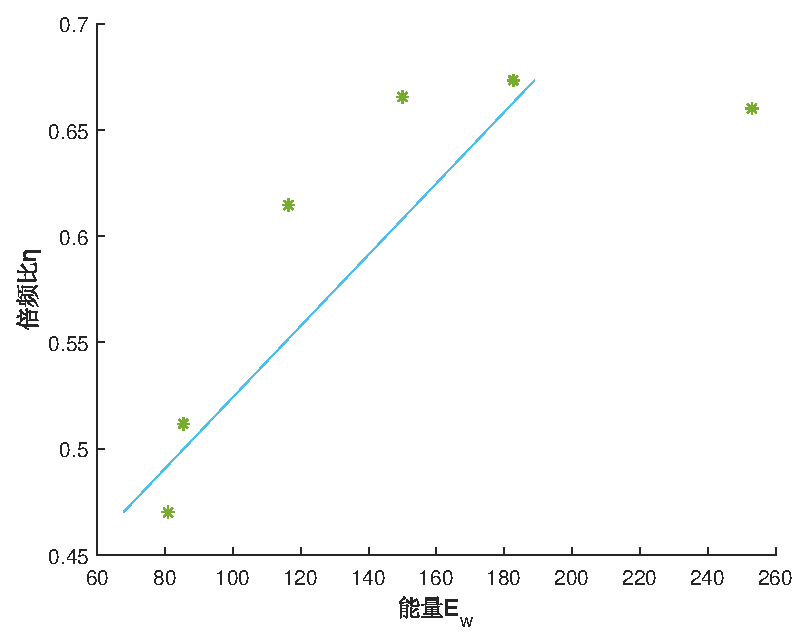
\includegraphics[width=13cm]{exp7.eps}
	\figcaption{KTP晶体的倍频特性拟合曲线}\label{exp7}
\end{center}
\subsection{实验结果分析}
	可以从图上看到,结果的线性程度并不是很高,如表2所示,我们分析了的原因大致跟实验六的类似,但是这个实验的误差会受到更多的影响,也就是因为实验六造成的误差的叠加。
	\begin{center}
		\tabcaption{拟合后曲线的参数}
		\begin{tabular}{|c|c|}
			\hline
			Linear model Poly&$f(x) = p_{1}*x + p_{2}$\\ \hline
			Coefficients (with 95\% confidence bounds)& $p_{1}$=0.001047,$p_{2}$ =  0.448  (0.2723, 0.6237)\\ \hline
			\multirow{4}{*}{Goodness of fit}&SSE: 0.01406\\
			&R-square: 0.627\\
			&Adjusted R-square: 0.5337\\
			&RMSE: 0.05929\\ \hline
		\end{tabular}
	\end{center}
\subsection{实验代码}
主程序代码如下,调用的函数可见实验6中的代码。
	\lstinputlisting[language={MATLAB},
numbers=left, numberstyle={\normalsize },	commentstyle=\color{red!50!green!50!blue!50}, 
frame=shadowbox, rulesepcolor=\color{red!20!green!20!blue!20}]
{code/exp7.m}
\section{注意事项}
\begin{enumerate}
	\item 不要用眼睛直视准直光源$He-Ne$光
	\item 开启激光电源前。戴上激光防护镜
	\item 泵浦氙灯易碎,不要碰及
\end{enumerate}
\section{思考题}
怎样获得更好的倍频效果?

实验也表明,并不是强光入射到非线性极化系数大的晶体就能获得良好的倍频效果,要想获得最佳的倍频效应,只有特定偏振方向的线偏振光以某一特定的角度入射时才能实现,不满足这个条件,倍频效果很差,甚至观察不到。这个特定角由相应匹配条件决定。
\section{参考文献}
\begin{description}
\item[1]. 雷仕湛,激光技术手册.科学出版社.北京.1992年.902-905页
\item[2]. 黄植文,黄显玲.激光实验.北京大学出版社.北京.1996年111-112页
\end{description}

\end{document}